\documentclass[11pt,a4paper]{article}

\usepackage{graphicx}

% ---- Idioma y tipografía
\usepackage[spanish]{babel}
\usepackage[T1]{fontenc}
\usepackage[utf8]{inputenc}  % (si usas XeLaTeX/LuaLaTeX, elimínala)
\usepackage{lmodern}
\usepackage{microtype}

% ---- Márgenes y diseño
\usepackage[a4paper,margin=2.2cm]{geometry}
\usepackage{parskip}

% ---- Enlaces
\usepackage[hidelinks]{hyperref}
\usepackage{bookmark}

% ---- Cabeceras y pies
\usepackage{fancyhdr}
\pagestyle{fancy}
\fancyhf{}
\renewcommand{\headrulewidth}{0.4pt}
\cfoot{\thepage}

% ---- Listas y símbolos
\usepackage{enumitem}
\setlist{itemsep=0.25em, topsep=0.3em}

% ---- Iconos y color
\usepackage{fontawesome5}
\usepackage{xcolor}
\usepackage[most]{tcolorbox}
\tcbuselibrary{breakable,skins}

% ---- Colores propios
\definecolor{uniPrimary}{HTML}{0A7AC3}
\definecolor{uniSoft}{HTML}{E9F4FB}
\definecolor{uniAccent}{HTML}{F5B700}
\definecolor{uniOK}{HTML}{2E7D32}
\definecolor{uniWarn}{HTML}{C62828}

% ---- Metadatos reutilizables
\newcommand{\asignatura}{MULTIMEDIA}
\newcommand{\tema}{TEMA 2 — Conceptos básicos sobre la compresión de datos}
\newcommand{\clase}{Clase 2}
\newcommand{\fecha}{\today}

% ---- Cabecera con metadatos
\lhead{\textsc{\asignatura}}
\rhead{\textbf{\tema}}

% ---- Estética de secciones
\usepackage{titlesec}
\titleformat{\section}{\Large\bfseries\color{uniPrimary}}{\thesection}{0.5em}{}
\titleformat{\subsection}{\large\bfseries}{\thesubsection}{0.5em}{}
\titleformat{\subsubsection}{\bfseries}{\thesubsubsection}{0.5em}{}

% ---- Cajas útiles
\newtcolorbox{ObjetivosBox}{
	title={\faBullseye\; Índice},
	colback=uniSoft,
	colframe=uniPrimary,
	enhanced, breakable,
	left=8pt,right=8pt,top=8pt,bottom=8pt,
	boxrule=0.8pt,
	fonttitle=\bfseries
}

\newtcolorbox{DefBox}{
	title={\faBook\; Definición},
	colback=white,
	colframe=uniAccent,
	enhanced, breakable,
	left=8pt,right=8pt,top=8pt,bottom=8pt,
	boxrule=0.8pt,
	fonttitle=\bfseries
}

\newtcolorbox{NotaBox}{
	title={\faStickyNote\; Nota},
	colback=white,
	colframe=uniPrimary,
	enhanced, breakable,
	left=8pt,right=8pt,top=8pt,bottom=8pt,
	boxrule=0.8pt,
	fonttitle=\bfseries
}

\newtcolorbox{RecordatorioBox}{
	title={\faBell\; Recordatorio},
	colback=uniAccent!15,
	colframe=uniAccent,
	enhanced, breakable,
	left=8pt,right=8pt,top=8pt,bottom=8pt,
	boxrule=0.8pt,
	fonttitle=\bfseries
}

\newtcolorbox{ChecklistBox}{
	title={\faTasks\; Tareas / Checklist},
	colback=white,
	colframe=uniPrimary,
	enhanced, breakable,
	left=8pt,right=8pt,top=8pt,bottom=8pt,
	boxrule=0.8pt,
	fonttitle=\bfseries
}

\newtcolorbox{ResumenBox}{
	title={\faHighlighter\; Resumen rápido (5 líneas)},
	colback=uniSoft,
	colframe=uniPrimary,
	enhanced, breakable,
	left=8pt,right=8pt,top=8pt,bottom=8pt,
	boxrule=0.8pt,
	fonttitle=\bfseries
}

\newtcolorbox{VocabBox}{
	title={\faLanguage\; Vocabulario clave},
	colback=white,
	colframe=uniPrimary,
	enhanced, breakable,
	left=8pt,right=8pt,top=8pt,bottom=8pt,
	boxrule=0.8pt,
	fonttitle=\bfseries
}

% =========================================================
\begin{document}

% ---- Cabecera de ficha de clase
{\large \textbf{\asignatura} \;—\; \textbf{\tema} \hfill}
\faUser\; Alumno/a: Alberto Díaz \hfill
\faChalkboardTeacher\; Profesor/a: Ana Fernández

\vspace{0.6em}

\begin{ObjetivosBox}
\begin{itemize}
	\item Comprender la estructura básica de un sistema de compresión.
	\item Diferenciar compresión con y sin pérdidas.
	\item Identificar los factores de diseño de un codificador.
	\item Conocer las principales técnicas de compresión.
\end{itemize}
\end{ObjetivosBox}

\tableofcontents

\section{Introducción a la compresión de datos}

\begin{DefBox}
Un sistema de compresión permite reducir el tamaño de los datos y, posteriormente, reconstruirlos para su uso.
\end{DefBox}

\section{Diseño de un codificador}

Cualquier algoritmo o técnica de compresión tiene dos partes:

\begin{itemize}
    \item Un sistema de \textbf{compresión} que toma una entrada $X$ y genera una representación $R$ que necesita menos espacio que $X$.
    \item Un sistema de \textbf{reconstrucción} que toma $R$ y construye $Y$, que es una aproximación de $X$.
\end{itemize}

\begin{figure}[!htbp]
    \centering
    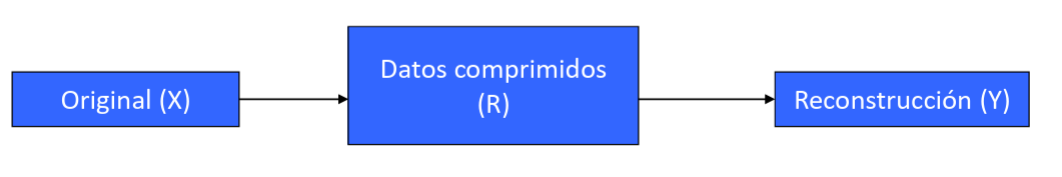
\includegraphics[width=0.85\linewidth]{resources/Coder_Decoder.png}
    \caption{Esquema de codificación y decodificación en un sistema de compresión.}
    \label{fig:coder-decoder}
\end{figure}

Un sistema de compresión consta de dos procesos: \textbf{codificación} y \textbf{decodificación}.

\begin{NotaBox}
Un sistema de compresión puede ser:
\begin{itemize}
    \item \textbf{Asimétrico}: el codificador es más complejo que el decodificador.
    \item \textbf{Simétrico}: el codificador y el decodificador tienen la misma complejidad.
    \item \textbf{Con pérdidas o irreversible}: aplicado a vídeo, audio, imagen.
    \item \textbf{Sin pérdidas o reversible}: aplicado a texto.
\end{itemize}
\end{NotaBox}

\subsection{Factores de diseño}

\begin{ChecklistBox}
Factores a considerar en el diseño de un codificador:
\begin{itemize}
    \item Retardo.
    \item Eficiencia (tasa de compresión).
    \item Complejidad.
    \item Calidad de la señal.
\end{itemize}
\end{ChecklistBox}

\begin{RecordatorioBox}
La mayoría de los estándares usan compresión con pérdidas, lo que permite alcanzar mayores tasas de compresión.
\end{RecordatorioBox}

\begin{figure}[!htbp]
    \centering
    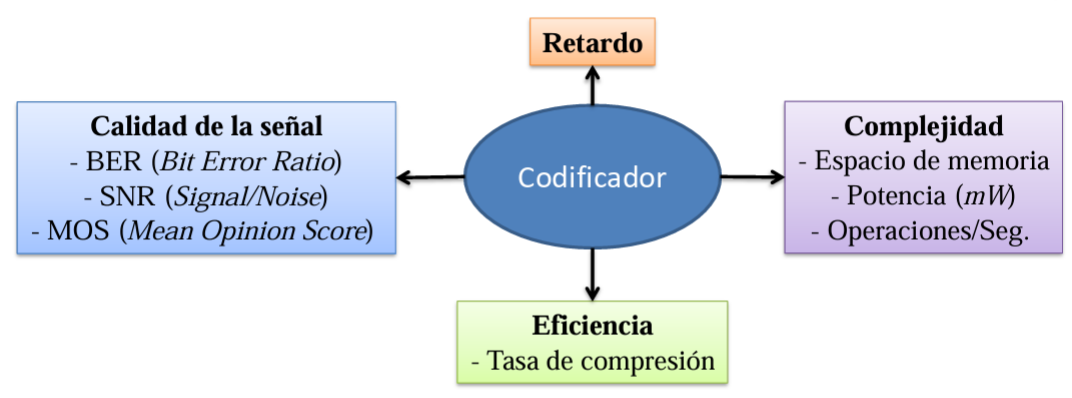
\includegraphics[width=0.85\linewidth]{resources/Coder_Metrics.png}
    \caption{Métricas típicas para evaluar un sistema de codificación.}
    \label{fig:coder-metrics}
\end{figure}

\section{Técnicas de compresión}

\subsection{Codificación entrópica}
Ejemplo: compresión \texttt{zip}.
Son independientes de las características del medio, por lo que se consideran universales.

\subsection{Codificación de fuente}
Codifica los datos basándose en las características del medio.
Suelen ser técnicas con pérdidas.
Permiten tasas de compresión elevadas.
Se aplican mediante codificadores de propósito específico.

\subsection{Codificación híbrida}
La mayoría de algoritmos pertenecen a este tipo.

\begin{ResumenBox}
Codificación entrópica es universal.
Codificación de fuente explota características del medio.
Codificación híbrida combina ambas.
\end{ResumenBox}

\begin{VocabBox}
\begin{itemize}
	\item \textbf{Compresión}: reducción del tamaño de los datos.
	\item \textbf{Codificación}: proceso de transformar los datos para reducir espacio.
	\item \textbf{Decodificación}: proceso de reconstrucción de los datos.
\end{itemize}
\end{VocabBox}

\subsection{Ejemplos}

\begin{figure}[!htbp]
	\centering
	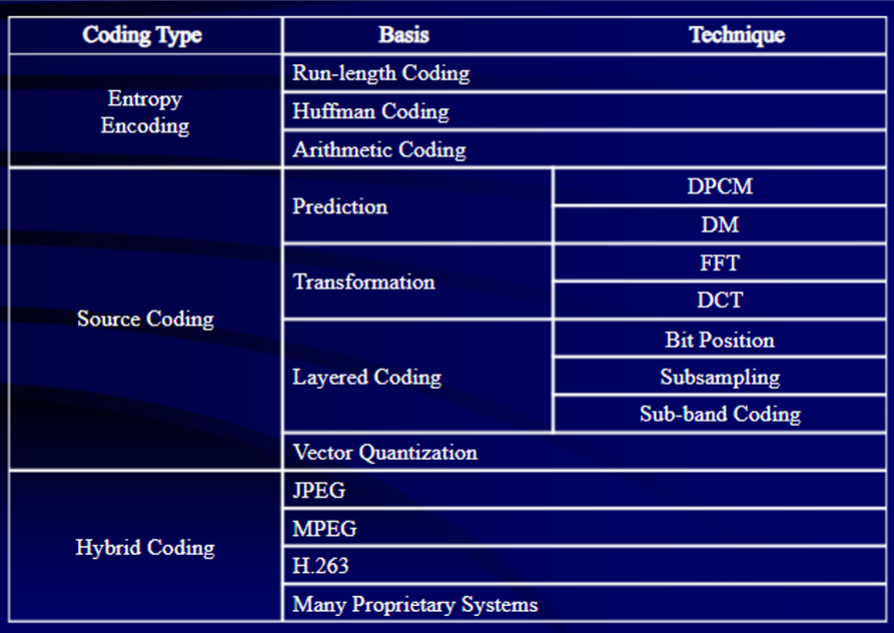
\includegraphics[width=0.8\linewidth]{resources/Compression_Types_Examples}
	\caption{Ejemplos de tipos de compresión: sin pérdidas, con pérdidas y mixtas.}
	\label{fig:compression-types-examples}
\end{figure}

\subsection{Compresión sin pérdidas}
\begin{itemize}
	\item \textbf{Técnicas estadísticas}
	\begin{itemize}
		\item \textbf{Codificación Huffman}:
		\item \textbf{Codificación aritmética}
	\end{itemize}
	\item \textbf{Técnicas basadas en diccionarios}
	\begin{itemize}
		\item \textbf{Lempel-Ziv-Welch (LZW)}:
	\end{itemize}
	\item \textbf{Técnicas predictivas}
	\begin{itemize}
		\item \textbf{Predicción y codificación del residuo}:
	\end{itemize}
\end{itemize}

\begin{NotaBox}
Los estándares suelen definir únicamente la parte de descompresión (decodificador).
\end{NotaBox}

\subsection{Compresión con pérdidas}

Se utiliza en ámbitos donde no es necesario reconstruir exactamente la señal original, como en:
\begin{itemize}
    \item Vídeos
    \item Audio
    \item Imágenes
\end{itemize}

\textbf{Técnicas:}
\begin{itemize}
    \item Cuantificación escalar
    \item Wavelets
    \item Transformación por bloques
\end{itemize}

\textbf{Estándares:}
\begin{itemize}
    \item JPEG
    \item JPEG 2000
    \item MPEG
\end{itemize}

\section{Conceptos Básicos}
\subsection{Calidad de un algoritmo de compresión}

Es necesario tener en cuenta:
\begin{itemize}
    \item Complejidad del algoritmo.
    \item Necesidad de memoria.
    \item Tiempo de ejecución.
    \item Cantidad de compresión.
    \item Grado de similitud entre la reconstrucción y los datos originales.
\end{itemize}

\subsection{Teoría de la información}

\begin{DefBox}
\textbf{Fuente:} par $(S, P)$

\begin{itemize}
    \item $S$ es un conjunto finito de mensajes denominado \textbf{alfabeto de la fuente}.
    \item $P : S \to [0,1]$ es una función de probabilidad que asigna a cada símbolo $s \in S$ su probabilidad de aparición $P(s)$.
    \item La probabilidad de un mensaje $s_1$ es $P(s_1)$.
\end{itemize}
\end{DefBox}

\begin{NotaBox}
Cuanto mayor sea la probabilidad de un mensaje, menor será su contenido de información.

Una fuente formada por mensajes de baja probabilidad aporta más información que una fuente compuesta por pocos mensajes de alta probabilidad.
\end{NotaBox}

\subsection{Cantidad de información}

La cantidad de información de un suceso $A$, con probabilidad de ocurrencia $P(A)$, se define como:

\[
I(A) = - \log_{2}\!\big(P(A)\big)
\]

La unidad de la información depende de la base del logaritmo:
\begin{itemize}
	\item Base 2: bits
	\item Base 10: Hartleys
	\item Base $e$: nats
\end{itemize}

Si 2 sucesos $A$ y $B$ son independientes, la cantidad de información conjunta es:
\[
I(A \cap B) = I(A) + I(B)
\]

\end{document}
